\chapter{Requisitos}

\section{Visão geral do sistema}
% nesta secção, apresentar o PRODUTO proposto: um sistema para apoiar projetos de I&D que incluem recolha de dados fisiológicos, que podem ocorrer em laboratório, como em ambulatório Identificar os atores envolvidos e as suas motivações 
O produto proposto é um sistema que permite a recolha de dados fisiológicos de pessoas e a respetiva revisão e investigação dos dados recolhidos. A recolha pode ocorrer em laboratório ou em ambulatório, isto é, os utilizadores podem recolher estes dados presencialmente ou remotamente. Um dos objetivos deste sistema é apoiar projetos de \gls{ID} que são cada vez mais importantes para reduzir a incerteza na utilização de determinadas tecnologias e ideias.
\par 
O sistema irá ser composto por uma aplicação móvel que tem como objetivo principal recolher dados dos sensores, e uma aplicação Web para visualizar esses dados recolhidos. O dispositivo com sensores utilizado poderá ser o \gls{VJ} e os dados fisiológicos recolhidos poderão ser a frequência cardíaca, \gls{ECG} e acelerómetro. Poderá ser utilizado este dispositivo pois como já fez parte de outros estudos, é um equipamento válido e permite recolher os tipos de dados que pretendemos. O sistema irá contemplar então dois atores distintos:
\begin{itemize}
  \item Revisor/Investigador que tem como objetivo rever dados inseridos pelos diferentes utilizadores
  \item Utilizador(alvo de estudo) que tem como função recolher dados vitais e acelerómetro para posteriormente serem revistos pelo revisor/investigador
\end{itemize}

\section{Casos de Utilização na Colheita de Dados}

Na figura \ref{f:usecaseandroidapp} podemos visualizar os casos de uso (cenários-objetivo) da aplicação móvel. O principal ator desta aplicação é o utilizador(alvo de estudo) que tem que recolher várias sessões de leitura para serem posteriormente analisadas e visualizadas por Investigadores/Revisores. 
\par
O ator pode estar envolvido nesta recolha de dados de duas maneiras diferentes. A primeira hipótese é fazer a recolha por ter o simples prazer de a realizar, pelo gosto e satisfação que lhe proporciona e por saber que está a ajudar a comunidade num caso de estudo. A segunda hipótese é fazer a recolha por ter algum problema físico, e querer com essa recolha seja analisado os seus dados fisiológicos, com o objetivo de o ajudar no seu futuro com as conclusões obtidas.

\begin{figure}[H]
  \centering
  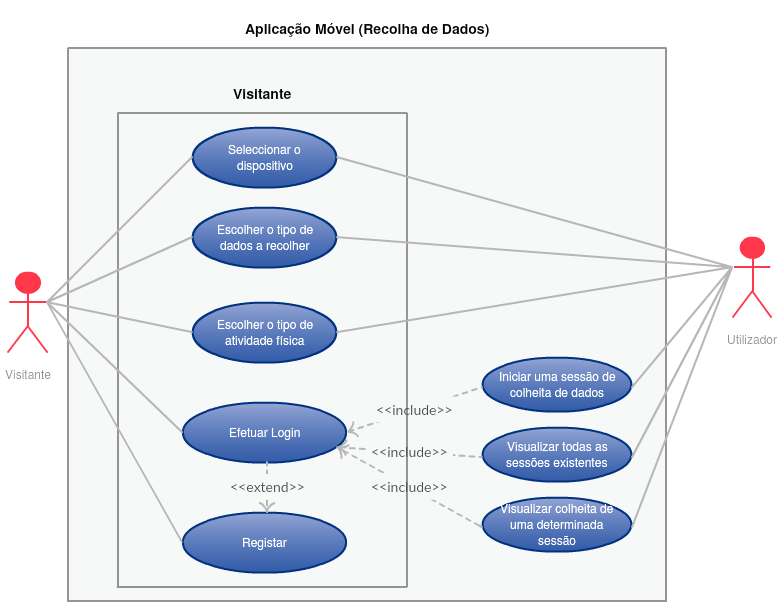
\includegraphics[width=0.9\textwidth]{imgs/app-and-usecase.PNG}
  \caption[Diagrama de casos de uso da aplicação móvel para colheita de dados]{Diagrama de casos de uso da aplicação móvel para colheita de dados}
  
  \label{f:usecaseandroidapp}
\end{figure}


\section{Casos de Utilização na Revisão de Dados}

Na figura \ref{f:usecasewebapp} podemos visualizar todos os casos de uso (cenários-objetivo) da aplicação web. O principal ator desta aplicação é o revisor/investigador que pode fazer uma revisão das várias sessões de recolha efetuadas pelos utilizadores.

\begin{figure}[H]
  \centering
  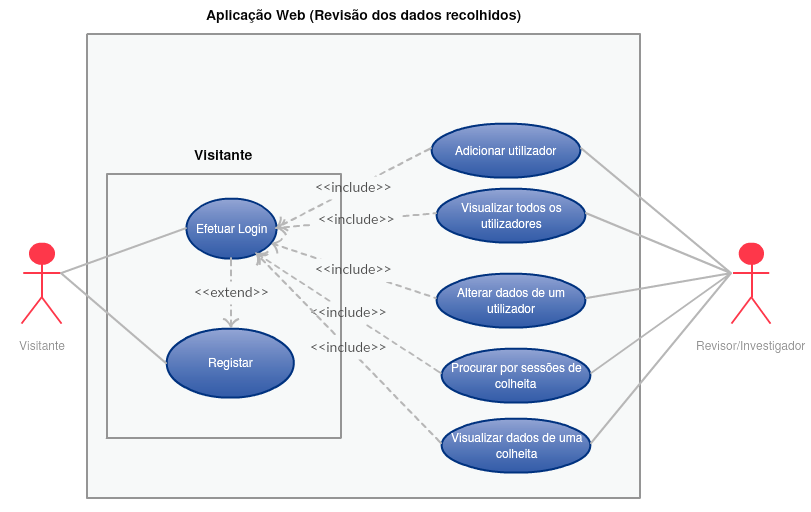
\includegraphics[width=0.9\textwidth]{imgs/app-web-usecase.PNG}
  \caption[Diagrama de casos de uso da aplicação web]{Diagrama de casos de uso da aplicação web}
  
  \label{f:usecasewebapp}
\end{figure}

\cleardoublepage